% !TEX root = ../main.tex
\subsection{Forwards MicroMegas Tracker} \label{ssec::forwardsmicromegastracker}
% --+ Micromegas +--------------------------------------------------------------
    \begin{figure}[b!]
        \centering\frame{
        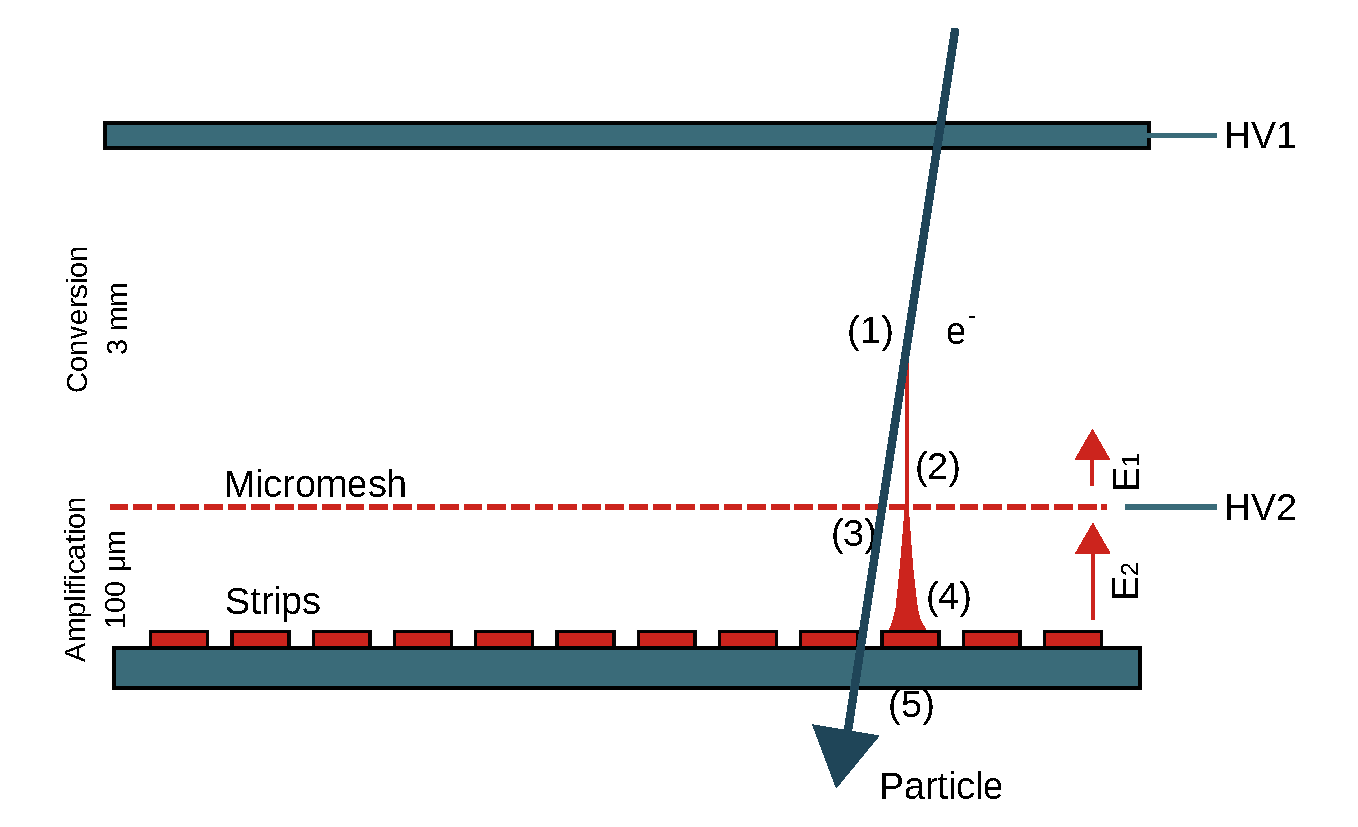
\includegraphics[width=\textwidth]{12fmtalign/img/10mm_principle.pdf}}
        \caption[MM working principle.]{MicroMegas working principle.}
        \label{fig::mm_principle}
    \end{figure}

    A Micro-Mesh Gaseous Detector or MicroMegas (MM) is a gaseous particle detector that follows from the well-known wire chambers.
    These type of detectors are commonly used in experimental physics for the detection of ionising particles.
    The MM detector offers very precise temporal and spatial resolution, to the order of 100 nanoseconds and below 100 micrometers \cite{giomataris1996}.

    The detector works by amplifying the charges that have been created by ionisation in the gas volume.
    It's volume is separated into two parts by a metallic micro-mesh placed less than 150 micrometers of the readouts electrode or strip.

    For clarity, this process is exhibited in figure \ref{fig::mm_principle}.

    While passing through the detector, a particle will ionise the gas atoms by pulling up an electron, creating an electron ion pair (1).
    An electric field is applied to the gas ($\text{E}_1$), allowing the electron to drift toward the amplification electrode (2) and the ion towards the cathode.
    As the electron crosses the mesh (3), it enters an intense electric field ($\text{E}_2$), causing an avalanche effect (4).
    This creates a significant signal at the readout strip (5), which can be then stored for reconstruction \cite{giomataris1996}.

% --+ Micromegas in CLAS12 +----------------------------------------------------
    Inside the CLAS12 detector, a wide array of tracking detectors are used to figure out the positions and momenta of a particle at various points in its trajectory.
    The closer these detectors are to the source of a particle, the more precision is obtained about the position and momentum at the vertex of the interaction, i.e. the point where the particle was produced.
    In an attempt to maximise this precision, the MicroMegas Vertex Tracker (MVT) in CLAS12 is placed as close to the target as possible, as can be seen in figure \ref{fig::mvt}.

    \begin{figure}[b!]
        \centering\frame{
        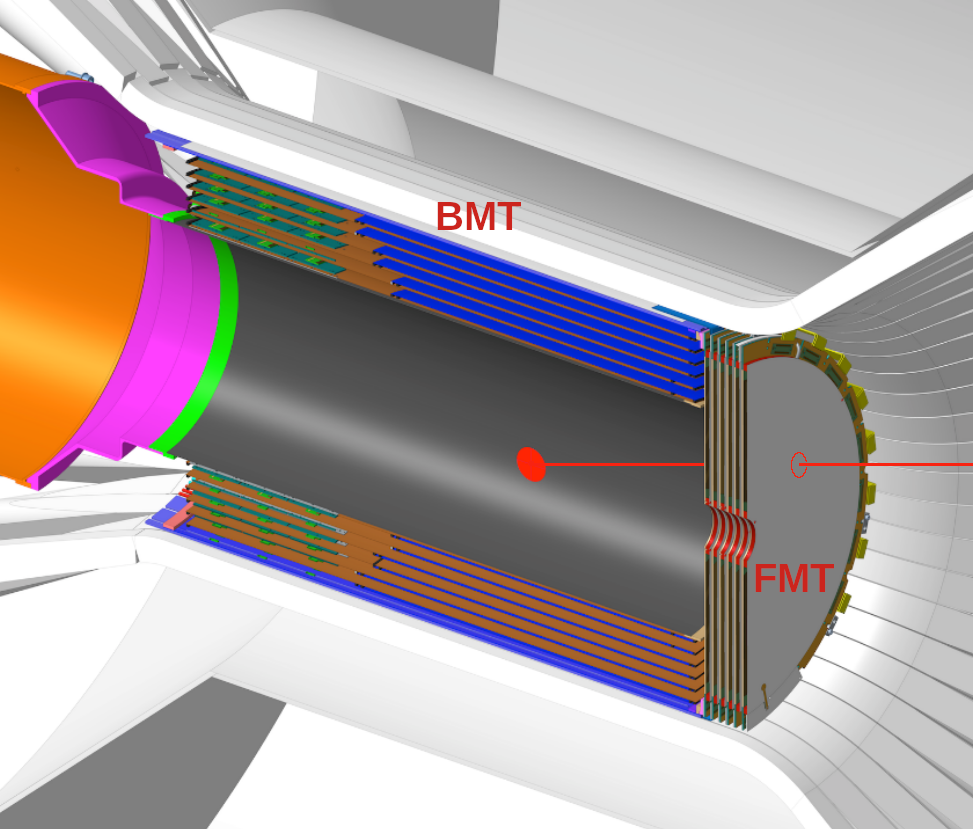
\includegraphics[scale=0.5]{12fmtalign/img/10mvt.png}}
        \caption[MVT detector.]{MVT detector. The red dot denotes the $z=0$ point in the beamline, the red line denotes an arbitrary track coming from that point, and the circumference in the Forward MicroMegas Tracker (FMT) denotes where that track produces a signal in an FMT layer.}
        \label{fig::mvt}
    \end{figure}

    Just as CLAS12 is divided into a central detector and a forward detector, the MVT is separated into two to maximise the angle coverage:
    The Barrel MicroMegas Tracker (BMT), a barrel tracker made of 18 cylindrical detectors arranged in 6 layers.
    This detector, in combination with the Silicon Vertex Tracker (SVT), covers the region from $35$ to $125\degree$ and greatly improves the polar angle resolution \cite{acker2020mvt}.

% --+ FMT +---------------------------------------------------------------------
    Then, the Forwards MicroMegas Tracker (FMT), which is made of six circular, flat detectors covering angles from $6$ to $29\degree$.
    In theory, it should improve the vertex resolution by a factor of $3$ to $10$ when compared to the Drift Chambers (DC) \cite{aune2009}.
    While the original design of the FMT included six layers, the current implemented detector has only three layers installed.
    This is due to technical difficulties and concerns regarding its Lorentz angle \cite{konczykowski2010}.

    Each of the three FMT layers has $1024$ readout strips, which follow a peculiar distribution, as can be seen in the image to the right of figure \ref{fig::fmt_geometry}.
    In addition, each layer's orientation differs by $60\degree$ to provide an accurate measurement in the xy-plane, as is shown in the image at the centre of the same figure \cite{acker2020mvt}.

    \begin{figure}[t]
        \centering\frame{
        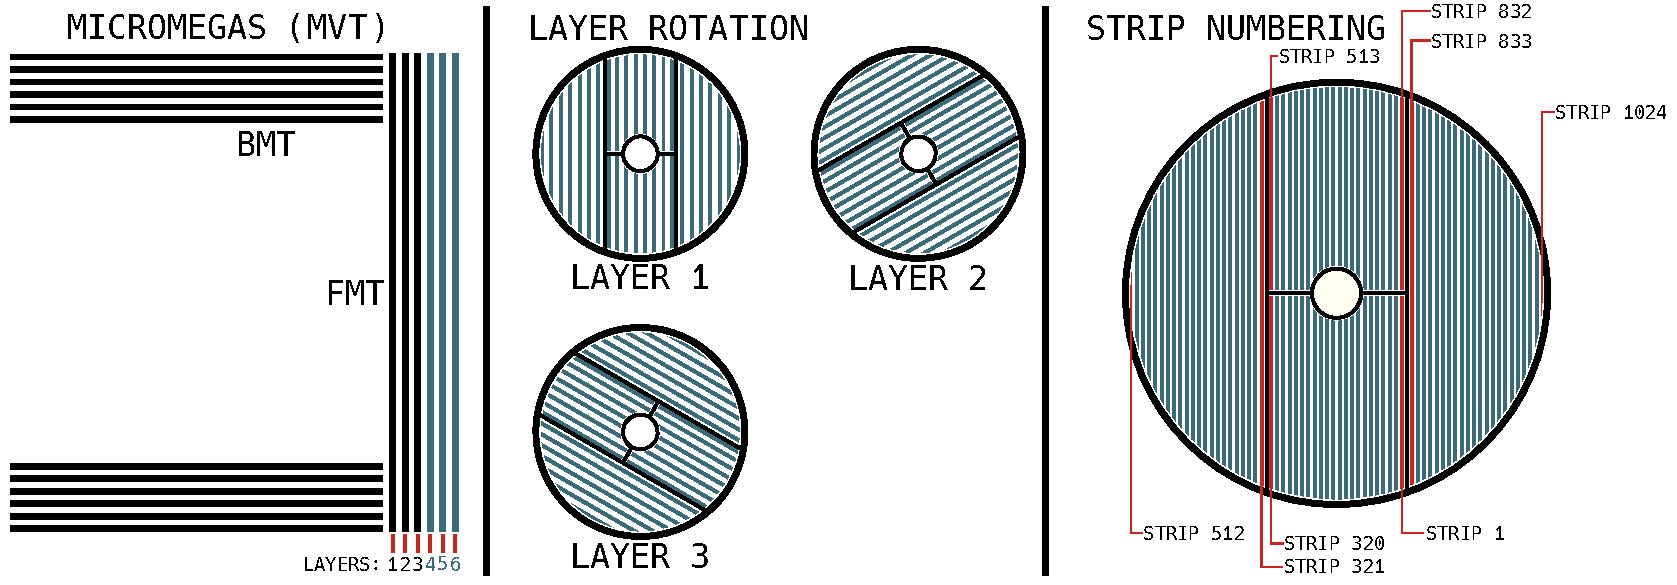
\includegraphics[width=\textwidth]{12fmtalign/img/10fmt_geometry.pdf}}
        \caption[FMT detector geometry.]{FMT detector geometry. The first picture shows the distribution of the BMT and FMT layers, the second the different angle of each FMT layer, and the third the readout strip distribution of each FMT layer.}
        \label{fig::fmt_geometry}
    \end{figure}

\subsubsection{FMT Reconstruction}
    \begin{wrapfigure}{r}{0.50\textwidth}
        \centering\frame{
        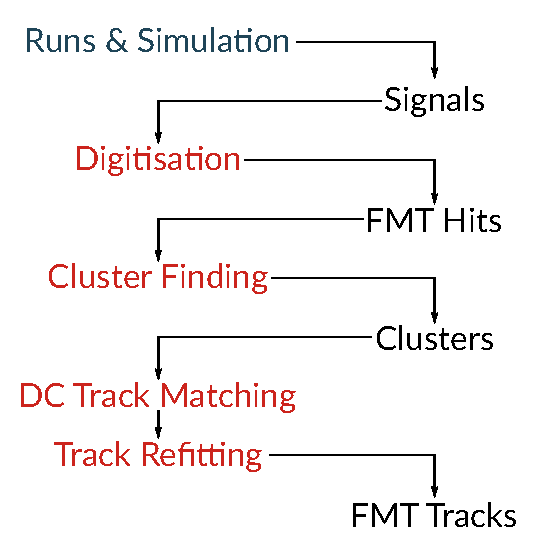
\includegraphics[width=\linewidth]{12fmtalign/img/10fmt_recon.pdf}}
        \caption[FMT reconstruction summary]{FMT reconstruction summary. Data taking is coloured blue, data in black, and processes in red.}
        \label{fig::fmt_recon}
    \end{wrapfigure}

    After a signal is detected on a readout strip and the data is stored, information is obtained from it from offline reconstruction.
    Being a tracker, FMT's reconstruction works in a fairly similar manner to DC's.

    First, after a signal is detected in a strip it is digitised, processed, and turned into an \textbf{FMT Hit}.
    A group of FMT hits is processed via a \textbf{Cluster Finding} algorithm, where a \textbf{Cluster} is defined as a group of hits that supposedly come from the same particle track.
    A group of clusters from different layers go through a \textbf{DC Track Matching} algorithm, where they are matched to DC tracks from DC Reconstruction.
    A \textbf{Track Refitting} algorithm is applied for each DC track using the clusters' data, updating them to re-fitted tracks, named \textbf{FMT tracks}.
    This whole process is summarised in figure \ref{fig::fmt_recon}.

\clearpage
